
%% LyX 2.2.3 created this file.  For more info, see http://www.lyx.org/.
%% Do not edit unless you really know what you are doing.
\documentclass[english]{beamer}
\usepackage[utf8x]{inputenc}
\setcounter{secnumdepth}{3}
\setcounter{tocdepth}{3}
\usepackage{amstext}
\usepackage{esint}
\usepackage{array}
\usepackage{amsfonts}
\usepackage{algorithm,algpseudocode}
\usepackage{caption}
\usepackage{subcaption}
\usepackage{stackengine}
\usepackage{multirow}
\usepackage{commath}

\newcommand{\indep}{\perp \!\!\! \perp}

\let\olditem\item
\renewcommand{\item}{%
\olditem\vspace{4pt}}
\DeclareMathOperator*{\argmax}{arg\,max}

\makeatletter
%%%%%%%%%%%%%%%%%%%%%%%%%%%%%% Textclass specific LaTeX commands.
 % this default might be overridden by plain title style
 \newcommand\makebeamertitle{\frame{\maketitle}}%
 % (ERT) argument for the TOC
 \AtBeginDocument{%
   \let\origtableofcontents=\tableofcontents
   \def\tableofcontents{\@ifnextchar[{\origtableofcontents}{\gobbletableofcontents}}
   \def\gobbletableofcontents#1{\origtableofcontents}
 }

%%%%%%%%%%%%%%%%%%%%%%%%%%%%%% User specified LaTeX commands.
\AtBeginDocument{%
   \let\origtableofcontents=\tableofcontents
   \def\tableofcontents{\@ifnextchar[{\origtableofcontents}{\gobbletableofcontents}}
   \def\gobbletableofcontents#1{\origtableofcontents}
 }% Choose how your presentation looks.
%
% For more themes, color themes and font themes, see:
% http://deic.uab.es/~iblanes/beamer_gallery/index_by_theme.html
%
\mode<presentation> {
  \usetheme{default}      % or try Darmstadt, Madrid, Warsaw, ...
  \usecolortheme{default} % or try albatross, beaver, crane, ...
  \usefonttheme{default}  % or try serif, structurebold, ...
  \setbeamertemplate{navigation symbols}{}
  \setbeamertemplate{caption}[numbered]
}

\let\@@magyar@captionfix\relax

\usepackage[english]{babel}
\usepackage{dsfont}

\newtheorem{prop}{Proposition}

\title[]{A User-Centric Approach to the Design and Consequences of Recommender Systems}
\author{Guy Aridor, Duarte Gon\c{c}alves, Shan Sikdar}
\institute{}
\date{October 4th, 2019}

\usepackage{babel}
\makeatother

\usepackage{babel}
\begin{document}
\begin{frame}
\titlepage
\end{frame}

\section{Motivation}
\begin{frame}
{Recommender Systems}
\begin{itemize}
\item How do consumers navigate a world where there are:
\begin{itemize}
\item thousands of movies on Netflix
\item millions of products on Amazon
\item billions of videos on YouTube
\end{itemize}
\pause
\item The industry response has been the development of \textit{recommender systems}
\begin{center}
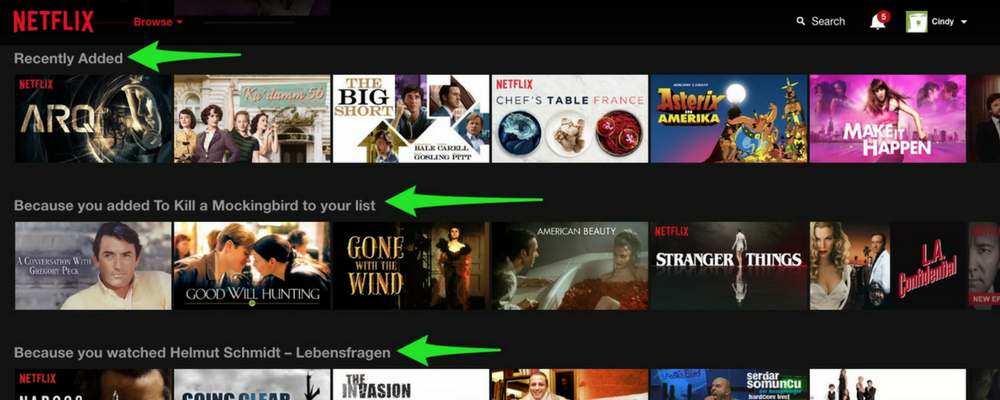
\includegraphics[scale=0.35]{netflix_rec}
\end{center}
\end{itemize}
\end{frame}
\begin{frame}
{Another Example}
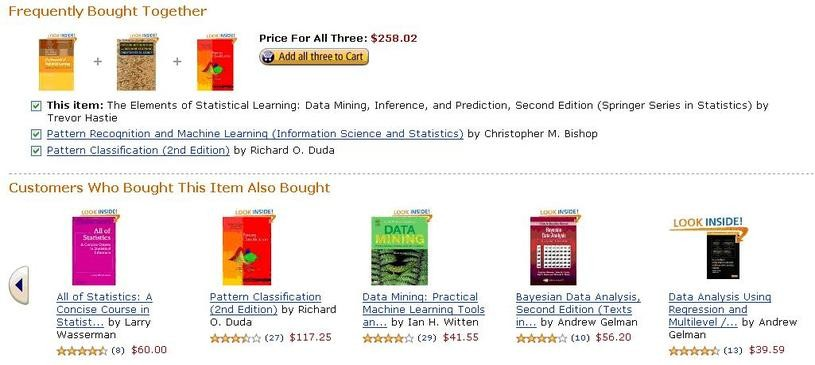
\includegraphics[scale=0.5]{rec_sys_example.jpg}
\end{frame}
%
\begin{frame}
{Recommendation and Consumer Choice}
\begin{itemize}
\item Recommender systems influence consideration and consumption choices of individuals
\begin{itemize}
\item 75\% of movies on Netflix
\item 35\% of page-views on Amazon
\item Aguiar and Waldfogel (2018) show that inclusion in Spotify's public recommendation playlists dramatically affects a song's likelihood of success
\end{itemize}
\pause
%\item Cremonesi, et. al (2013), Nguyen et. al (2014), Adomavicius et. al (2013), and many others show that recommender systems impact consumer choices and shape preferences
\item But how does recommendation change how individuals make decisions?
\end{itemize}
\end{frame}
%
\begin{frame}
{Three Motivating Questions}
\begin{enumerate}
    \item Can platforms with market power use recommendation as a form of steering?
    \pause
    \item Are recommender systems having unintended social consequences (e.g. filter bubbles, user homogenization)?
    \pause
    \item How can we design useful recommendation systems?
\end{enumerate}
\pause
\vspace{1cm}
\textbf{This paper}: First-order concern is to understand how consumers make decisions in environments where recommender systems are deployed
\end{frame}
%

\begin{frame}
{Model Demonstration I}
\begin{center}
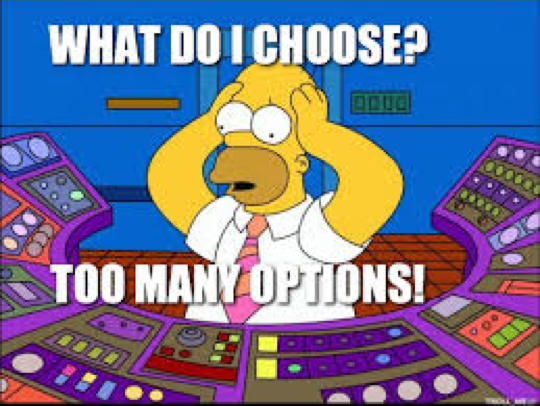
\includegraphics[scale=0.5]{homer} \\
How to pick a movie on Netflix? a video on YouTube?
\end{center}
\pause
\textbf{Ingredient 1}: Long-lived consumers that face large choice sets
\begin{itemize}
    \item Challenge is that can only consume a small portion of the overall choice set 
\end{itemize}
\end{frame}
%
\begin{frame}{Model I - Setting}
\begin{itemize}
    \item Each individual faces a choice set $\mathcal{J} = \{ 1, ... N \}$ of $N$ items
    \item Consumes $T << N$ of these items
    \item $u_{in} = v_{in} + \beta v_{n}$
    \begin{itemize}
    \item $v_{in}$ - idiosyncratic component of utility
    \item $v_{n}$ - common value component
    \item $\beta$ controls how ``predictable" a user's preferences are given other's preferences
    \item Users learn true $u_{in}$ after consumption
    \end{itemize}
\end{itemize}
\end{frame}
%
\begin{frame}
{Model Demonstration II}
\begin{center}
Which would you pick?
\vspace{0.2cm}
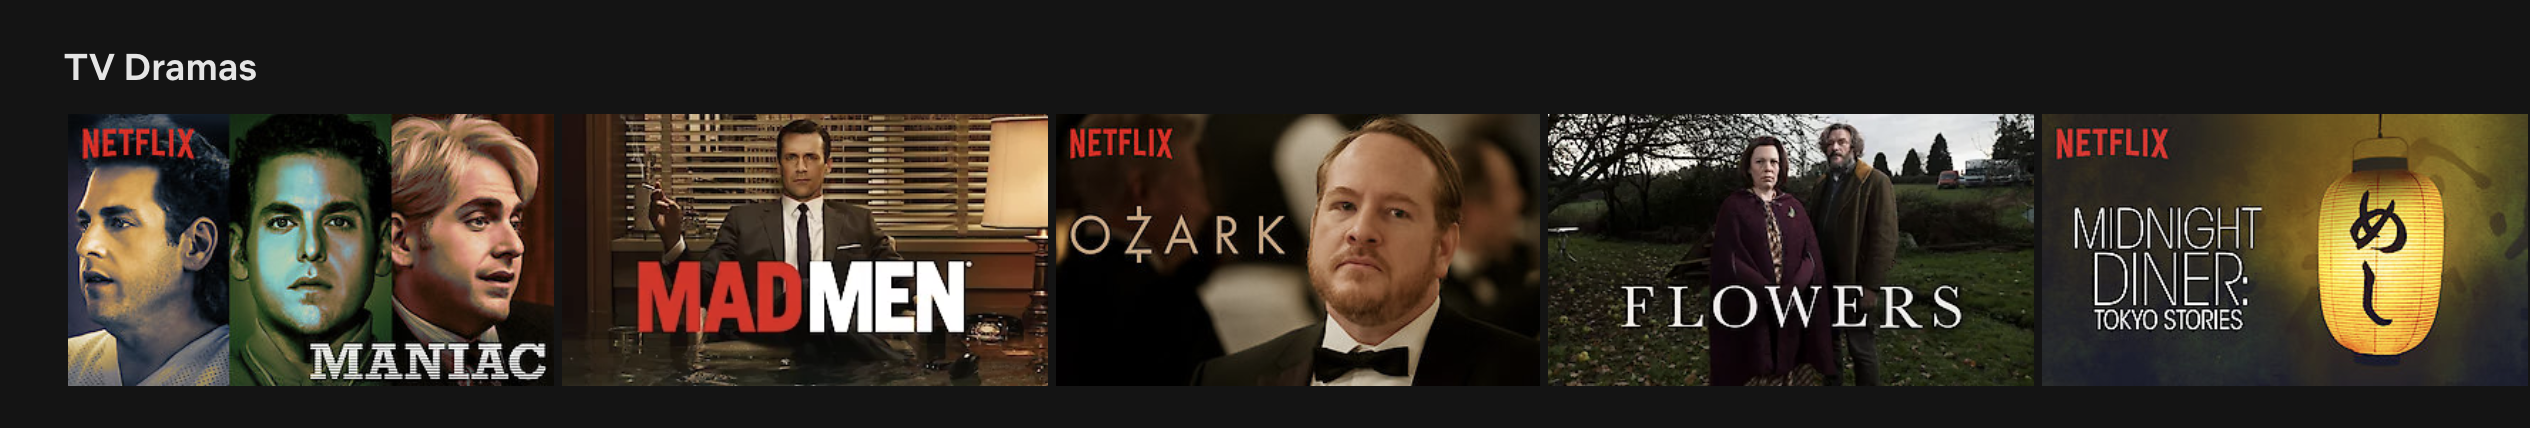
\includegraphics[scale=0.25]{netflix.png}
\end{center}
\pause
\vspace{0.5cm}
\textbf{Ingredient 2}: Uncertainty over realized utility of items
\end{frame}
%
\begin{frame}{Model II - User Beliefs}
\begin{itemize}
    \item Distributions of $V$ and $V_i$
    \begin{itemize}
    \item $V_i \indep V$
    \item $V_i \sim \mathcal{N}(\overline{V_{i}}, \Sigma_i)$
    \item $V \sim \mathcal{N}(\overline{V}, \Sigma)$, $\overline{V} = 0$
    \item Why Gaussian?
    \begin{itemize}
        \item Recall Gaussian distributions form a conjugate prior - closed form Bayesian updating
        \item Allows intuitive way to model correlation structure
    \end{itemize}
    \end{itemize}
    \item Prior beliefs for individual $i$ are drawn $\overline{v}_{in} \sim \mathcal{N}(0, \overline{\sigma}^2)$
    \item CARA preferences: $\delta(n) \sim \mu_n - \frac{1}{2}\gamma \Sigma_{nn}$
\end{itemize}
\end{frame}
%
\begin{frame}
{Model Demonstration III}
\begin{center}

\includegraphics[scale=0.21]{john_wick}

\includegraphics[scale=0.11]{john_wick_2} \\
\end{center}
Suppose you ended up watching \textit{John Wick} and it was:
\begin{itemize}
    \item Good? \pause Watch \textit{John Wick: Chapter Two}? \pause
    \item Bad? \pause Watch something very different?
\end{itemize}
\pause
\textbf{Ingredient 3}: Learning spillovers - consumption gives information about similar items (e.g. similarity-based generalization)
\end{frame}
%
\begin{frame}{Model III - Informational Spillovers}
\begin{itemize}
    \item Conceptually, products are evenly space on a circle
    \begin{itemize}
    \item $d(n, m) = \min \{ \abs{m - n}, N - \abs{m - n} \}$
    \end{itemize}
    \item $(n, m)$ entry in $\Sigma_{i}$ is given by $\rho^{d(n, m)} \sigma_{i}^{2}$ (same with $\Sigma$)
    \item Combined with distance measure - $(n, n+1)$ entry is $\rho$, etc.
    \item higher $\rho$ $\implies$ larger spill-overs
    \item higher $d(n, m) \implies$ smaller spill-overs
\end{itemize}
\end{frame}
%
\begin{frame}{Model IV - Recommendation}
\begin{itemize}
    \item Model recommendation as providing information to users to reduce uncertainty
    \item Three recommendation regimes:
    \begin{enumerate}
        \item No Recommendation: Users get no information
        \item Recommendation: Recommender knows true $V$ + idiosyncratic beliefs = personalized recommendation
        \item Oracle: Ex-post (full information) optimal consumption path
    \end{enumerate}
    \end{itemize}
\end{frame}
%
\begin{frame}{Model Evaluation}
\begin{itemize}
    \item Focus on numerical simulation of our model over $P$ populations of $I$ individuals
    \item For each population, average over consumers to get ``representative" consumer from population
    \item Reported results are over a dataset of representative populations over a fine grid of parameter values
\end{itemize}
    
\end{frame}
\begin{frame}
{Question #1: Filter Bubbles}
\begin{center}
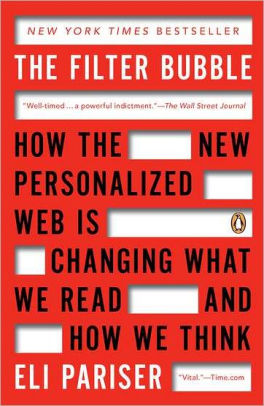
\includegraphics[scale=0.2]{filter_bubble}
\end{center}
Do personalized recommender systems lead users into increasingly narrow portions of the product space?
\begin{itemize}
    \item Empirical studies find little evidence for this due to recommender systems in various domains (news, movie consumption)
    \item Find that this happens \textit{without recommendation}
\end{itemize}
\textbf{Our model}: Learning spillovers induce over-consumption around ``local maxima" (amplified when users are risk-averse)
\end{frame}
%
\begin{frame}{Filter Bubbles - No Correlation}
\begin{center}
    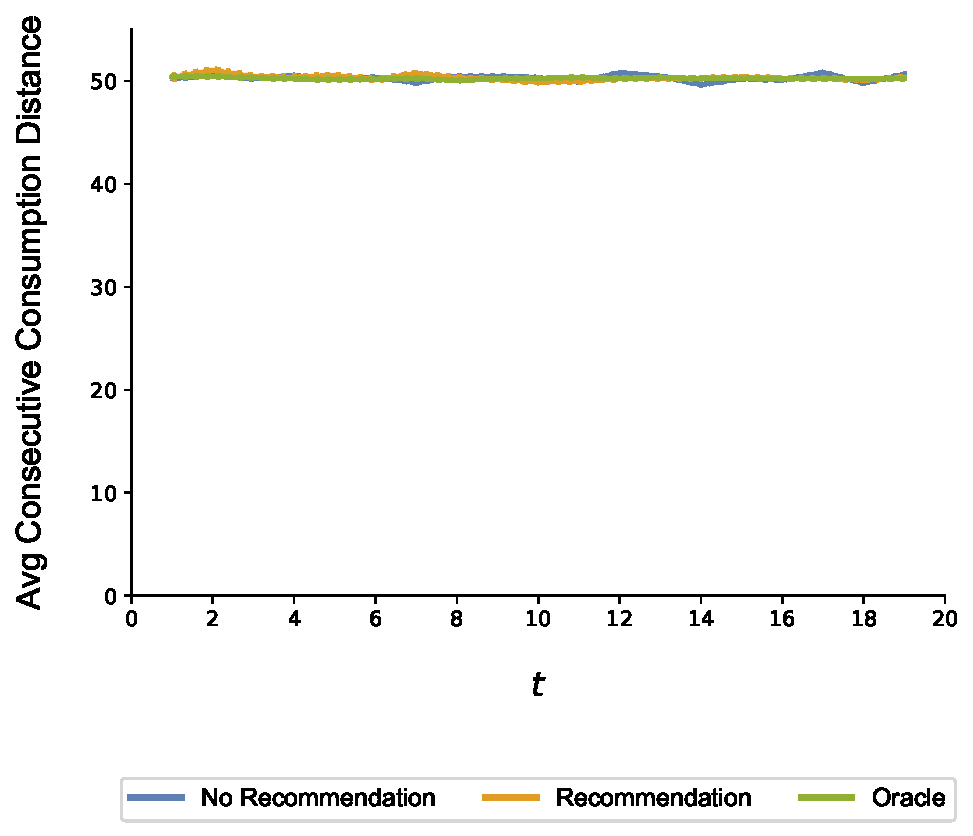
\includegraphics[scale=0.5]{consumption_dist_N_200T_20no_correlation}
\end{center}
\end{frame}
%
\begin{frame}{Filter Bubbles - Overall}
\begin{center}
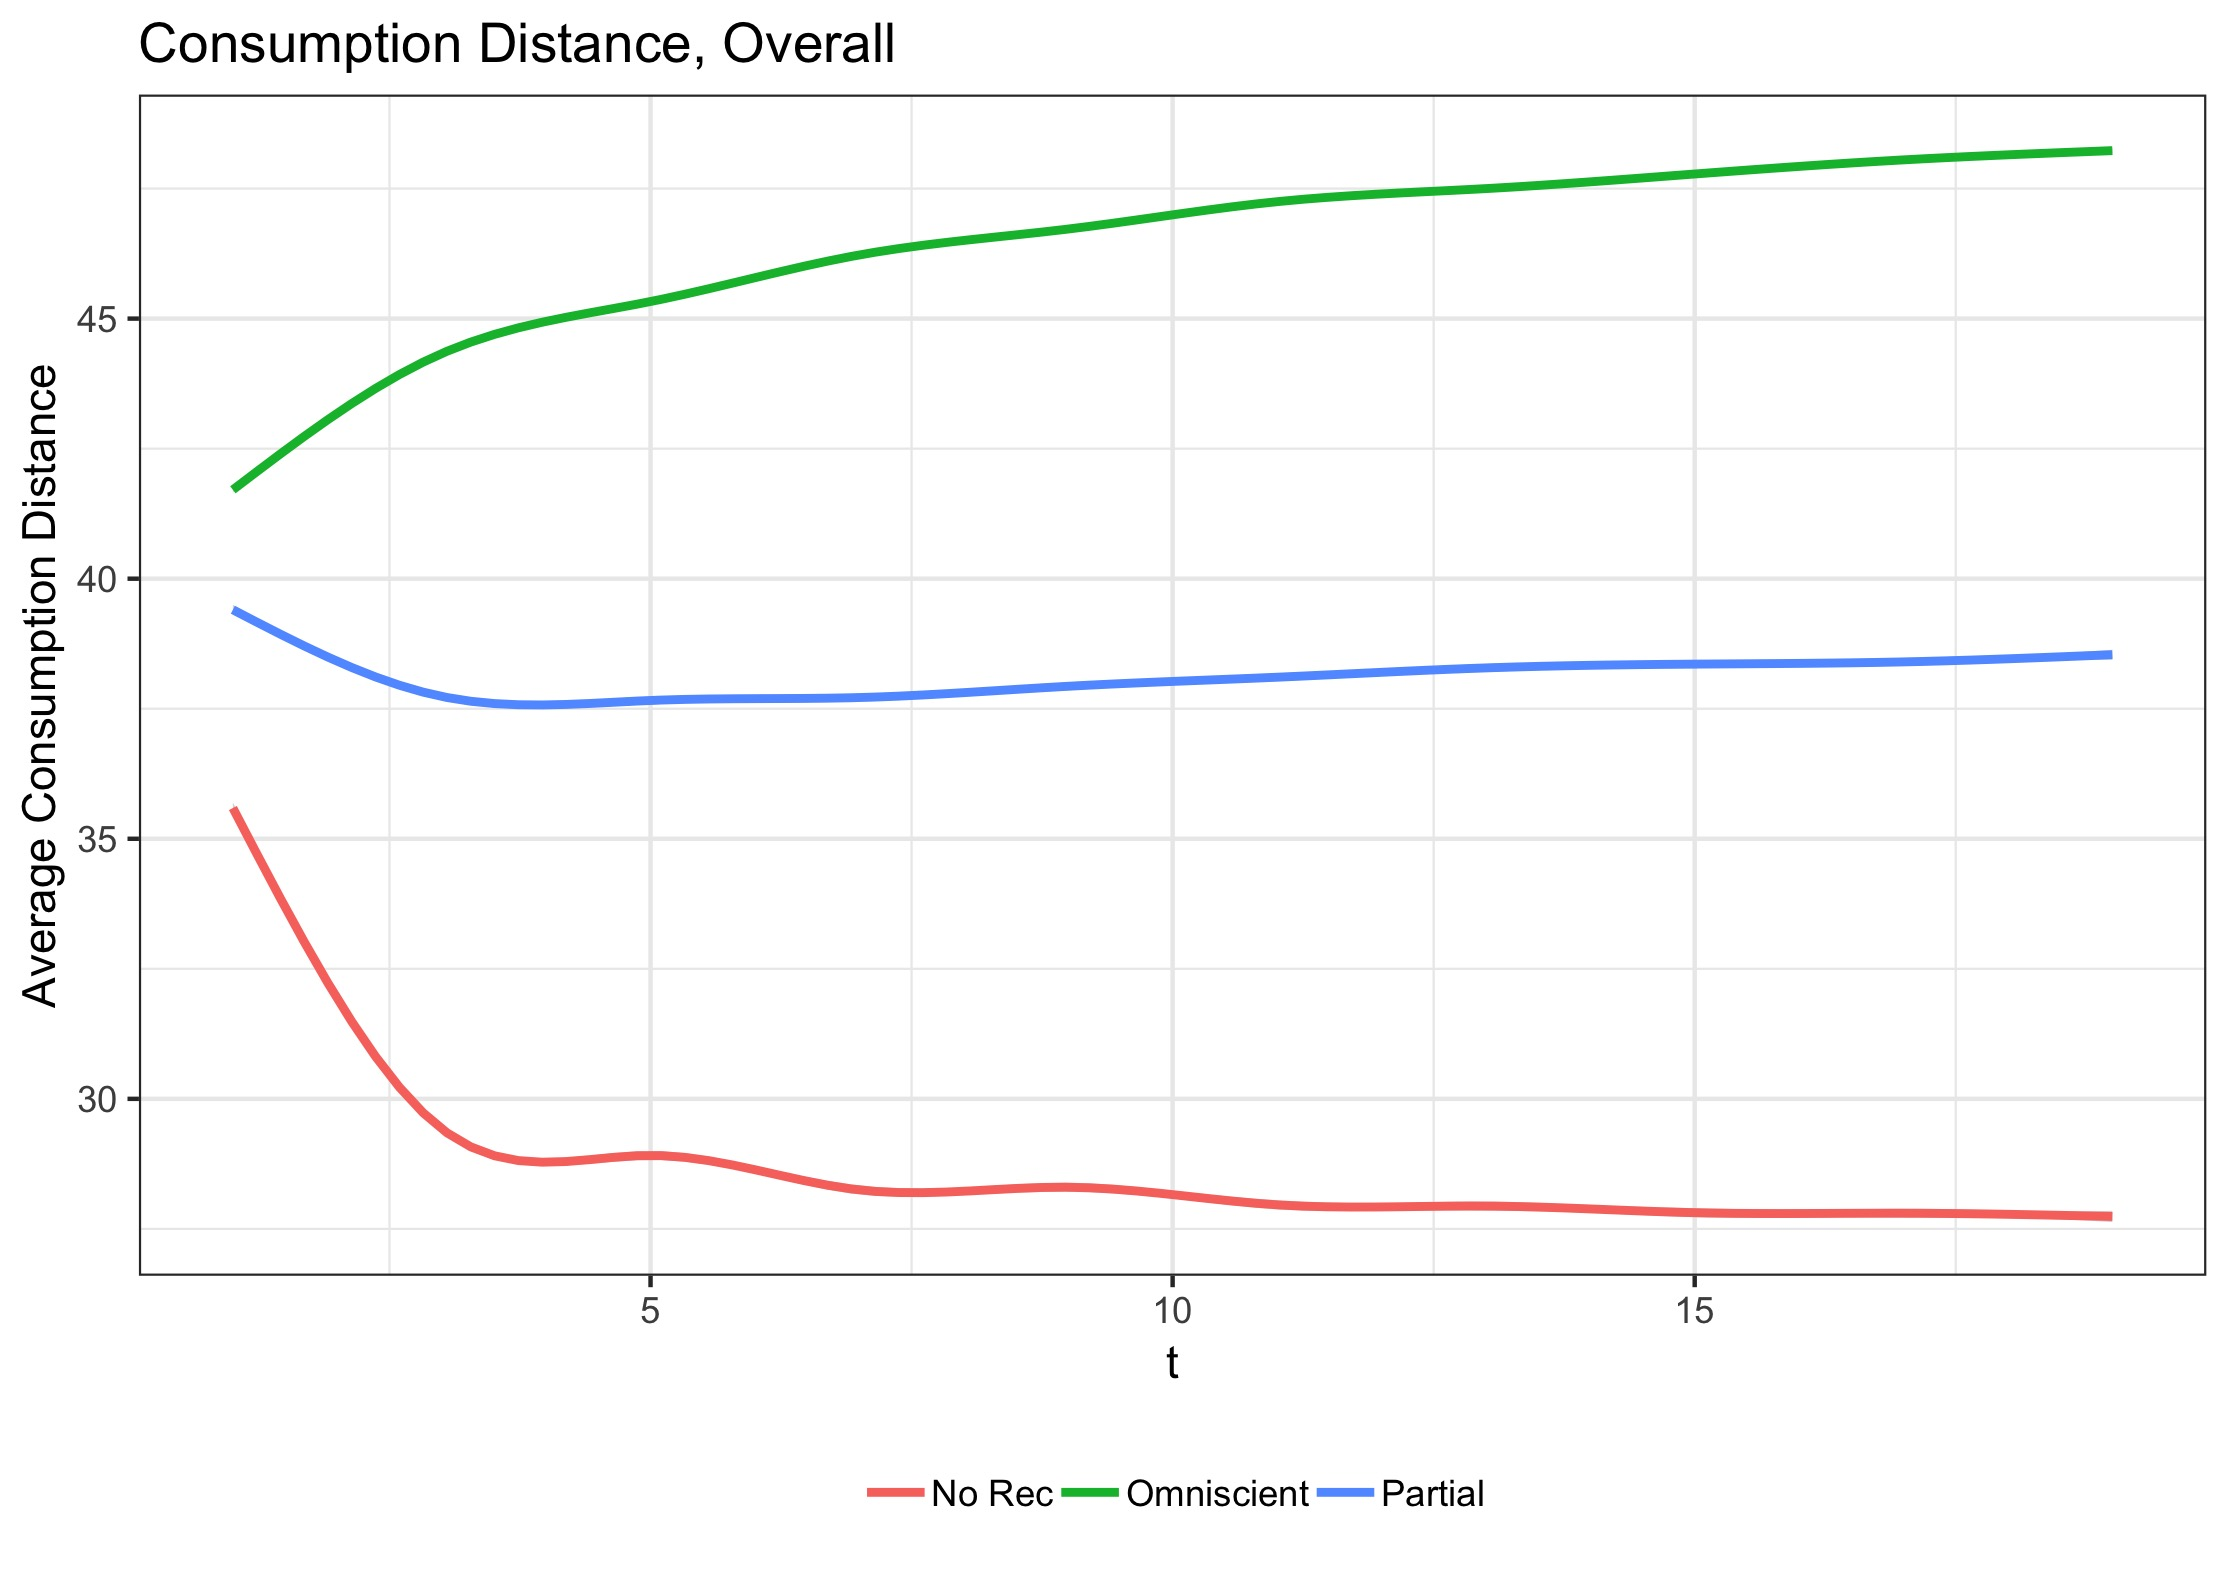
\includegraphics[scale=0.1]{consumption_dist_N_200T_20_overall}
\end{center}
\end{frame}
%
\begin{frame}{Filter Bubbles - Increasing $\rho$}
\begin{center}
    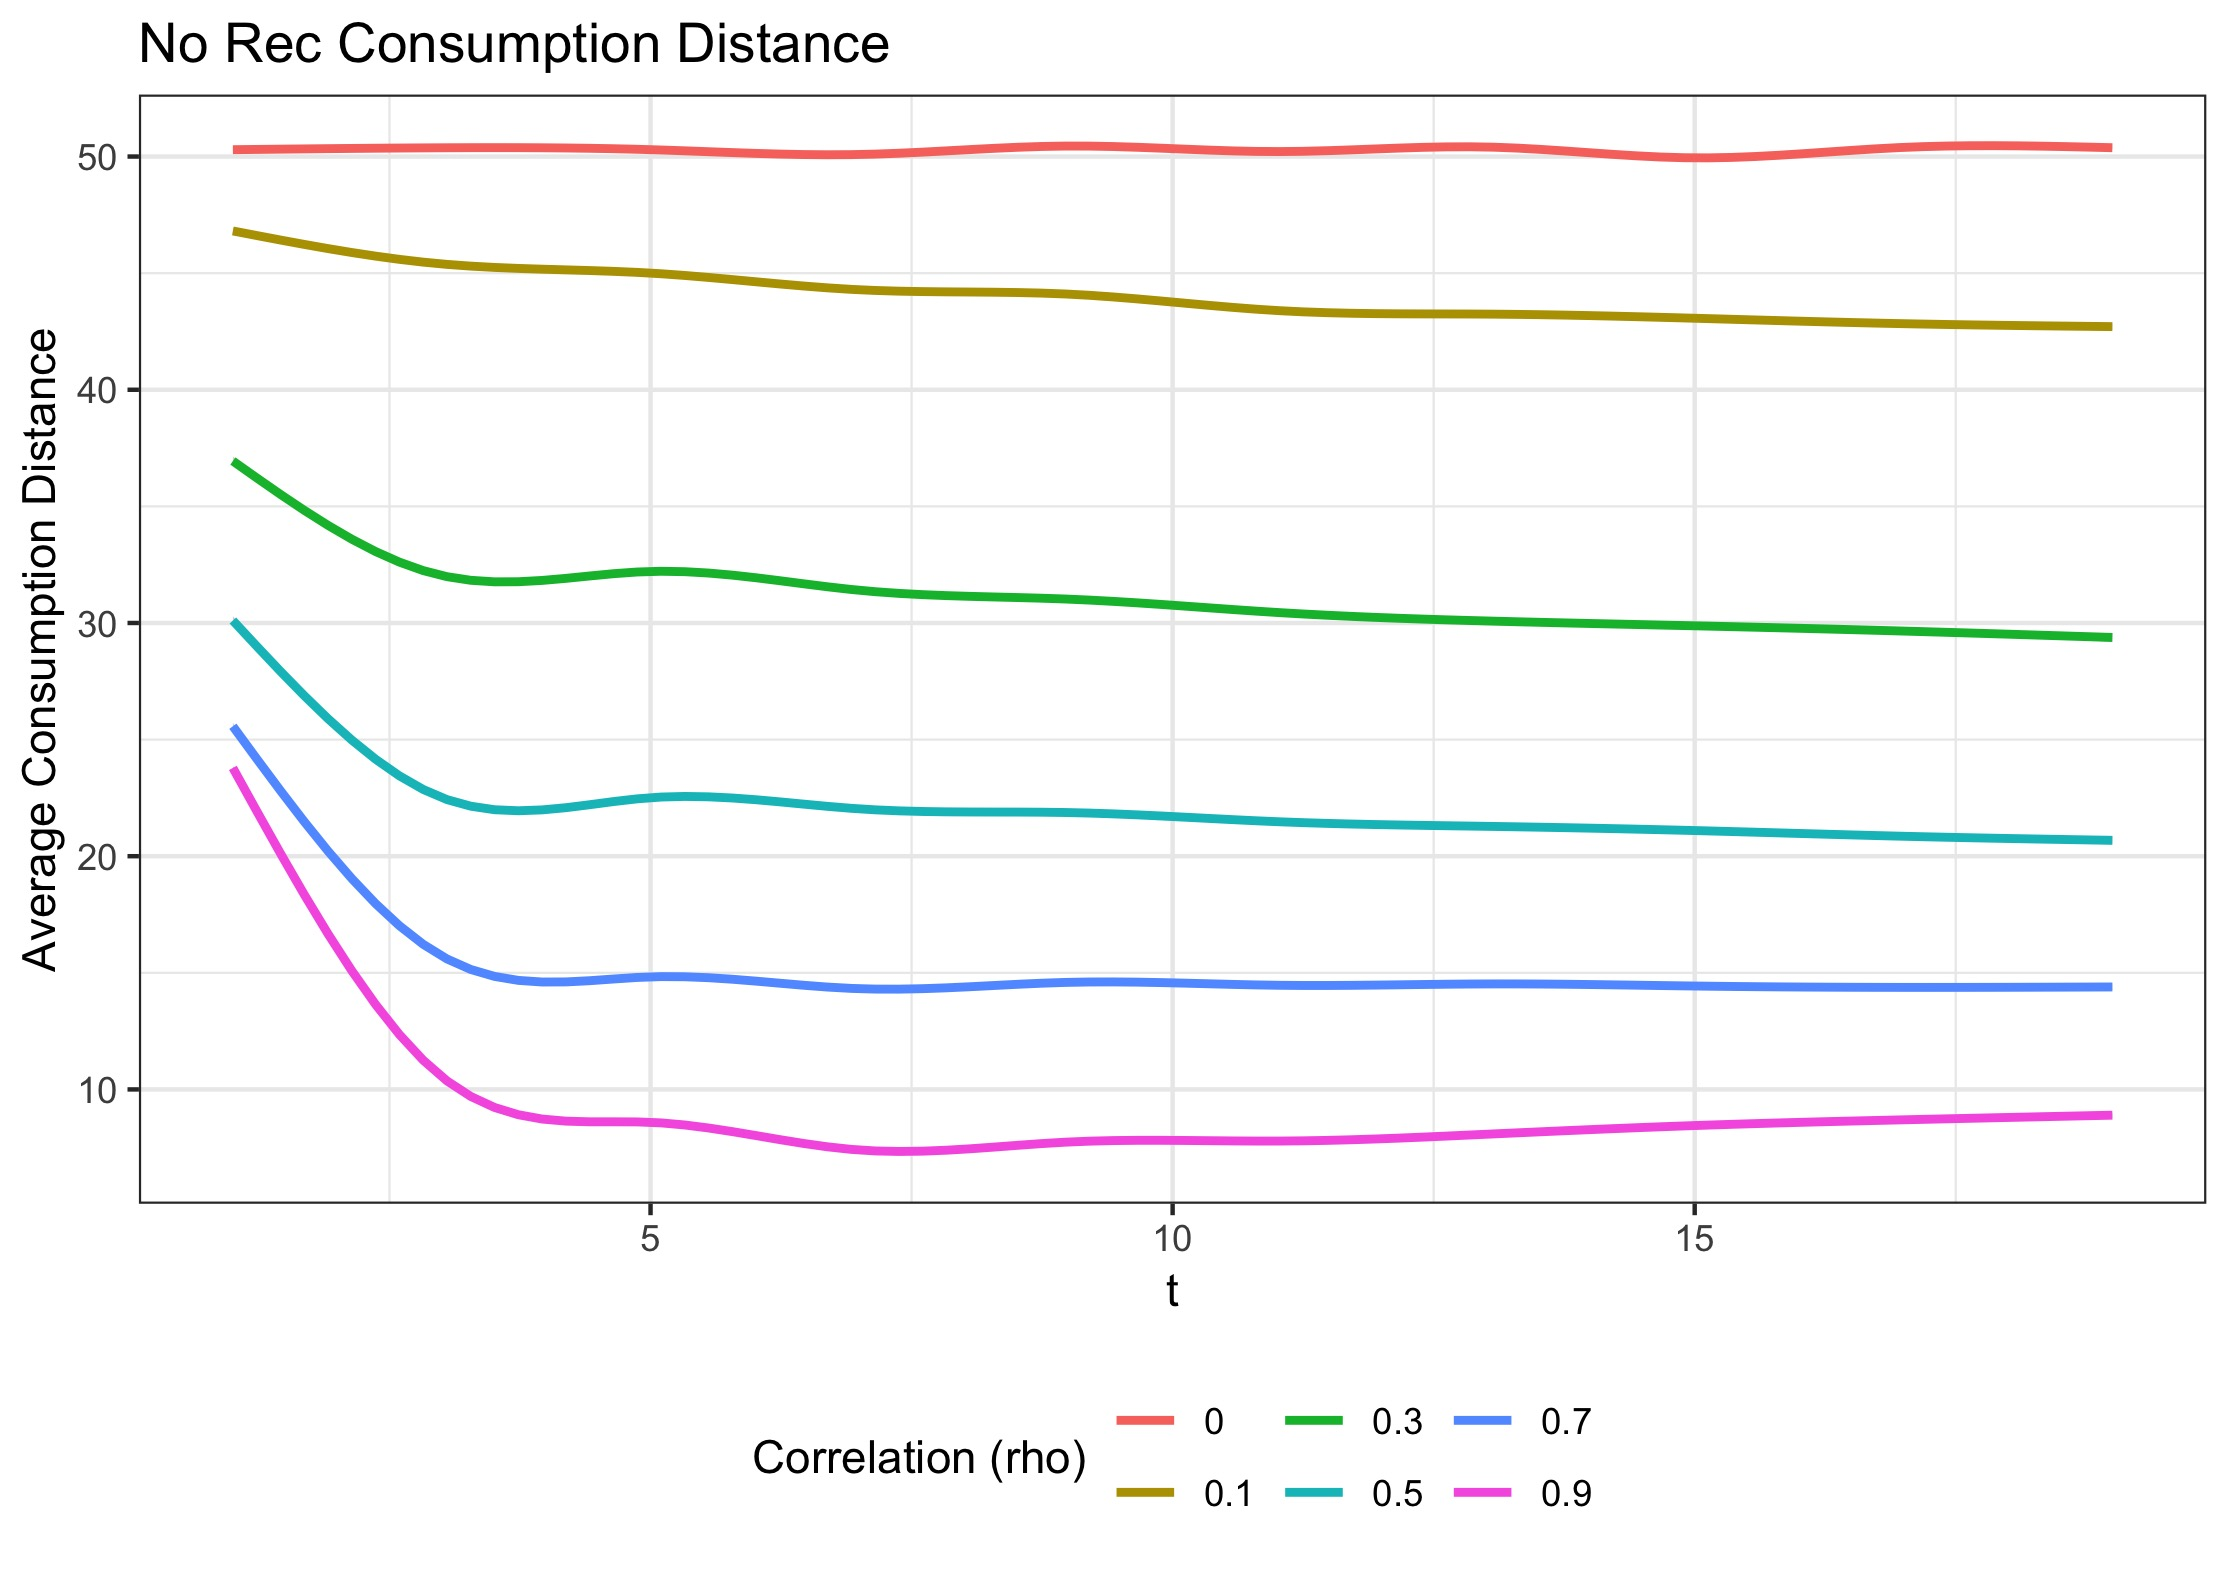
\includegraphics[scale=0.07]{consumption_dist_N_200T_20_no_rec_rho.jpeg}
    \pause
    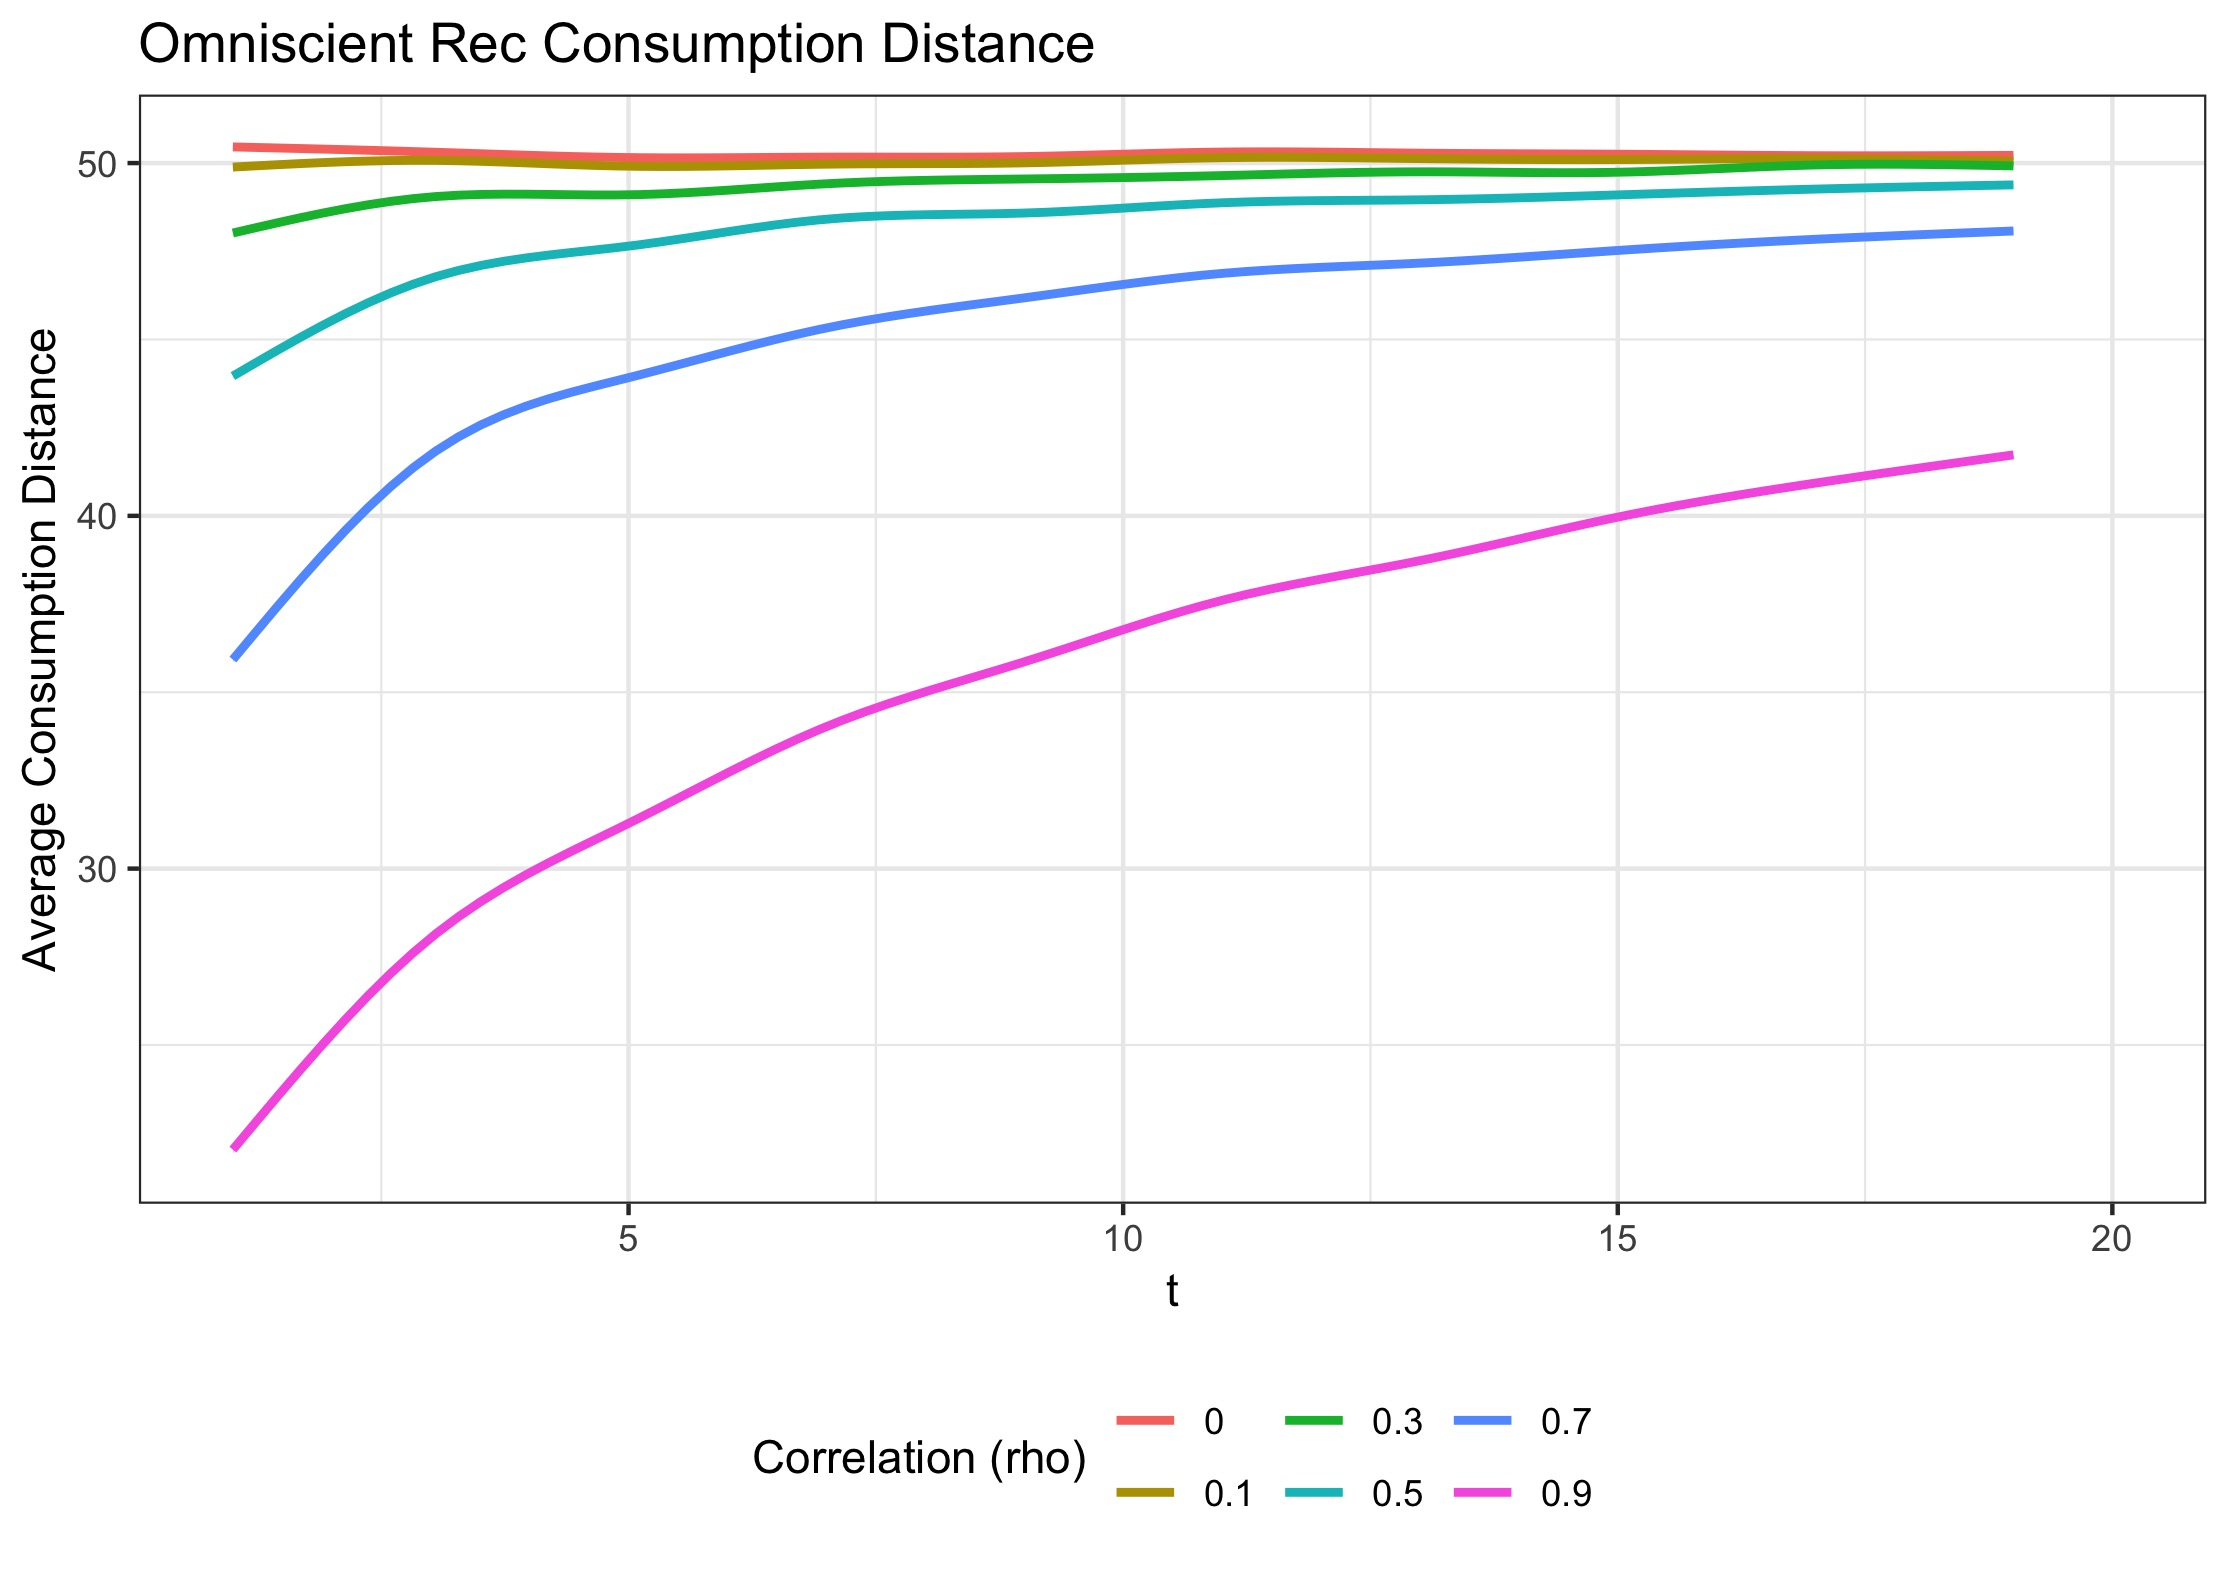
\includegraphics[scale=0.07]{consumption_dist_N_200T_20_omni_rho}
\end{center}
    
\end{frame}
\begin{frame}{Question #2: Product Diversity}
Is aiming for product diversity a good goal for recommender systems?\\
\vspace{0.5cm}
\textbf{Our model}: Without recommendation, diversity can be \textit{negatively correlated} with consumer welfare
\begin{itemize}
    \item Recall the John Wick example: high diversity can be induced by many bad experiences and lead users to jump all over the product space
    \item Strong risk-aversion weakens this, but leads to users being stuck in ``bad" portions of the product space
    \item Recommendation weakens this since it coordinates users to consume in ``good" parts of the product space
\end{itemize}
\end{frame}
%
\begin{frame}{Diversity, Welfare vs $\rho$}
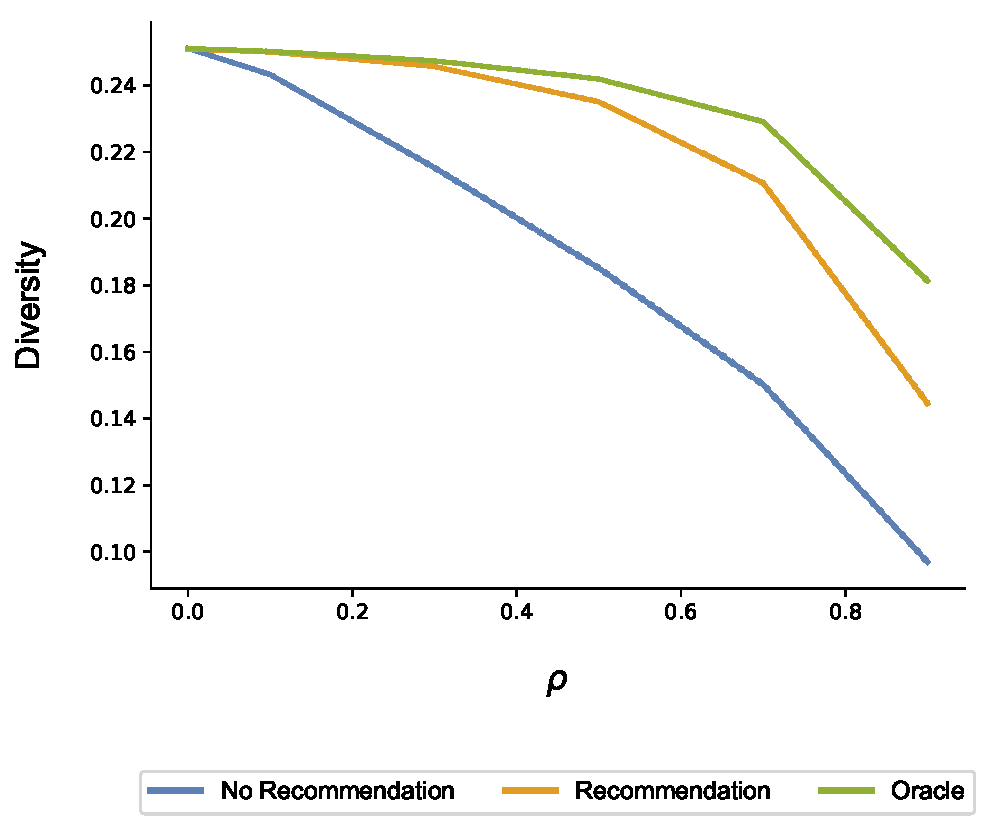
\includegraphics[scale=0.3]{rho_diversity_N_200_T_20} \pause
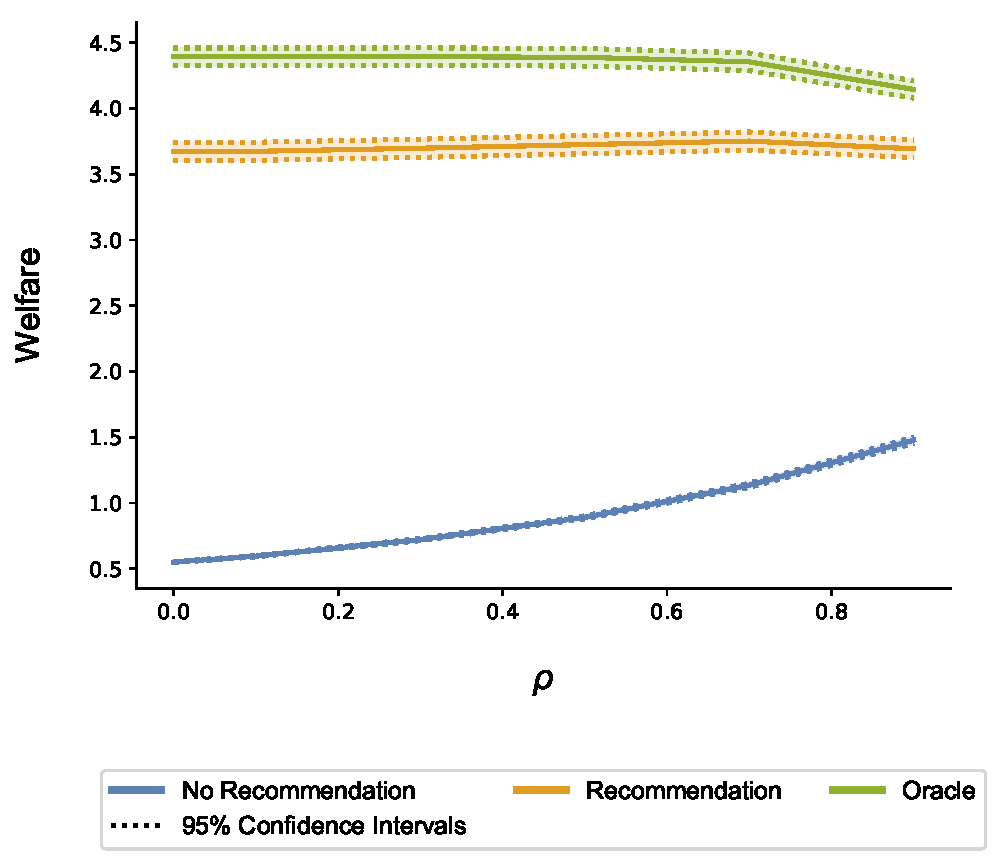
\includegraphics[scale=0.3]{rho_welfare_N_200_T_20}
\end{frame}
\begin{frame}{Diversity vs Welfare - No Recommendation}
    \begin{center}
        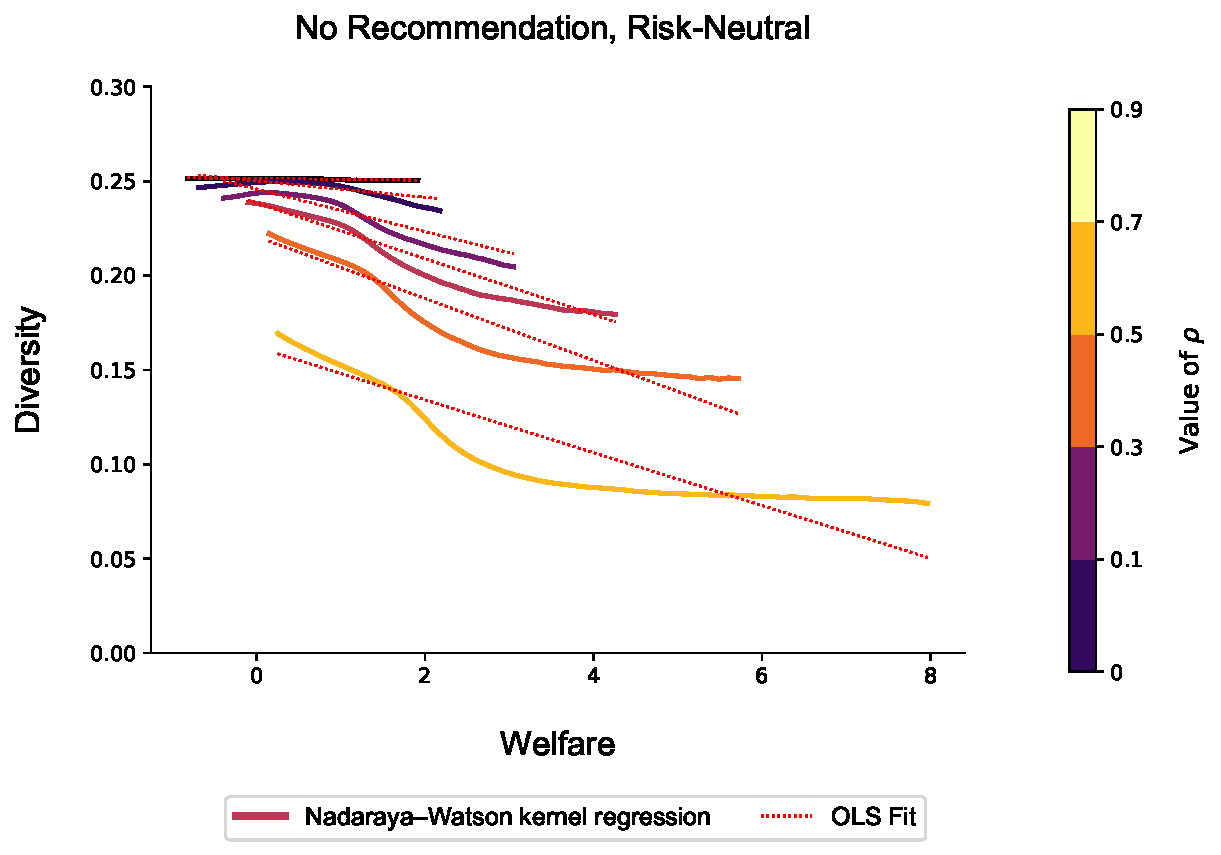
\includegraphics[scale=0.3]{diversity_welfare_no_risk_aversion.pdf}
        \pause
        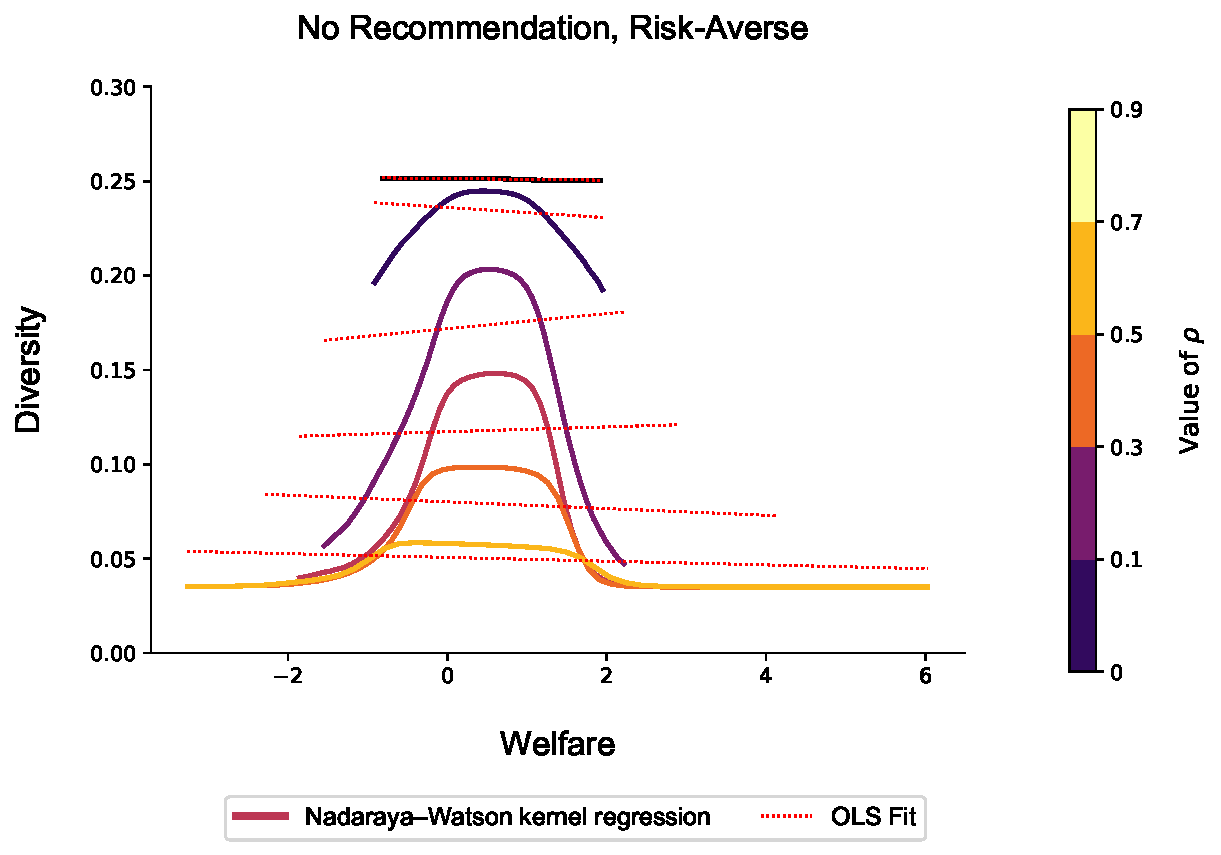
\includegraphics[scale=0.3]{diversity_welfare_high_ra}
    \end{center}
\end{frame}
%
\begin{frame}{Question #3: User Homogeneity}
Do recommender systems induce users to consume similar sets of items? \\
\vspace{0.5cm}
\textbf{Our model}: 
\begin{itemize}
    \item Oracle has a small amount of homogeneity
    \item No recommendation has no homogeneity - random exploration around the product space
    \item Recommendation coordinates users around same goods - high homogeneity
\end{itemize}
\end{frame}
%
\begin{frame}{Homogeneity - Varying $\beta$}
\begin{center}
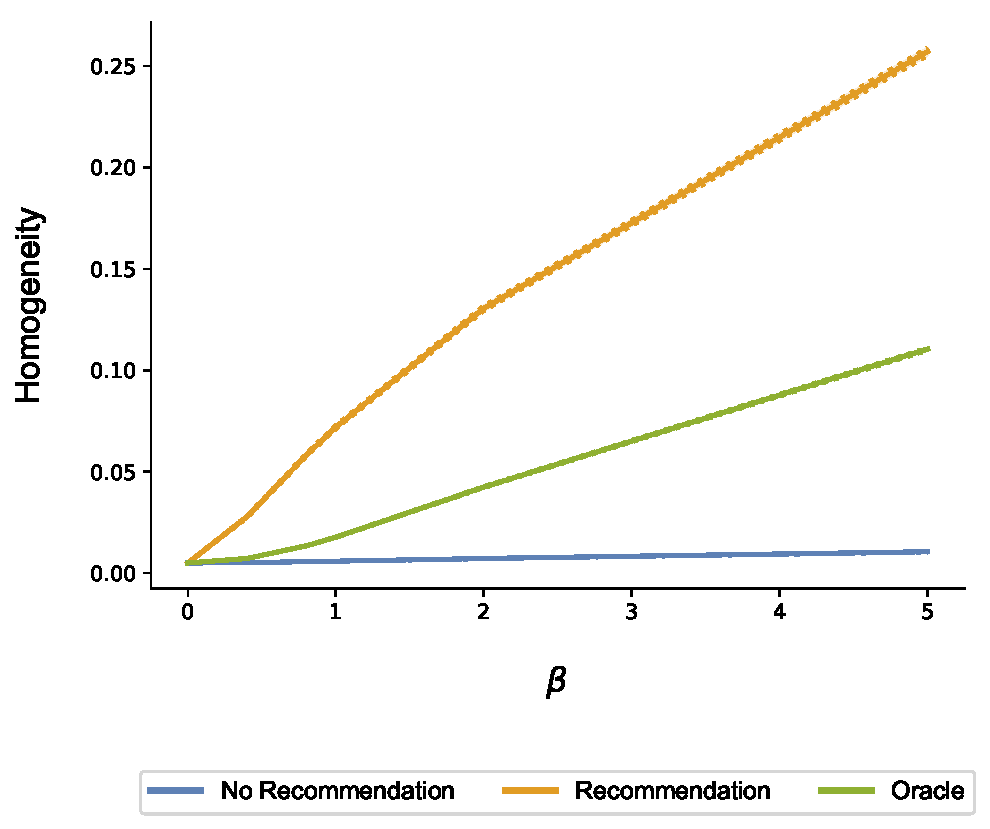
\includegraphics[scale=0.5]{beta_homogeneity_N_200_T_20}
\end{center}
\end{frame}
%
\begin{frame}{Homogeneity - Varying $\rho$}
\begin{center}
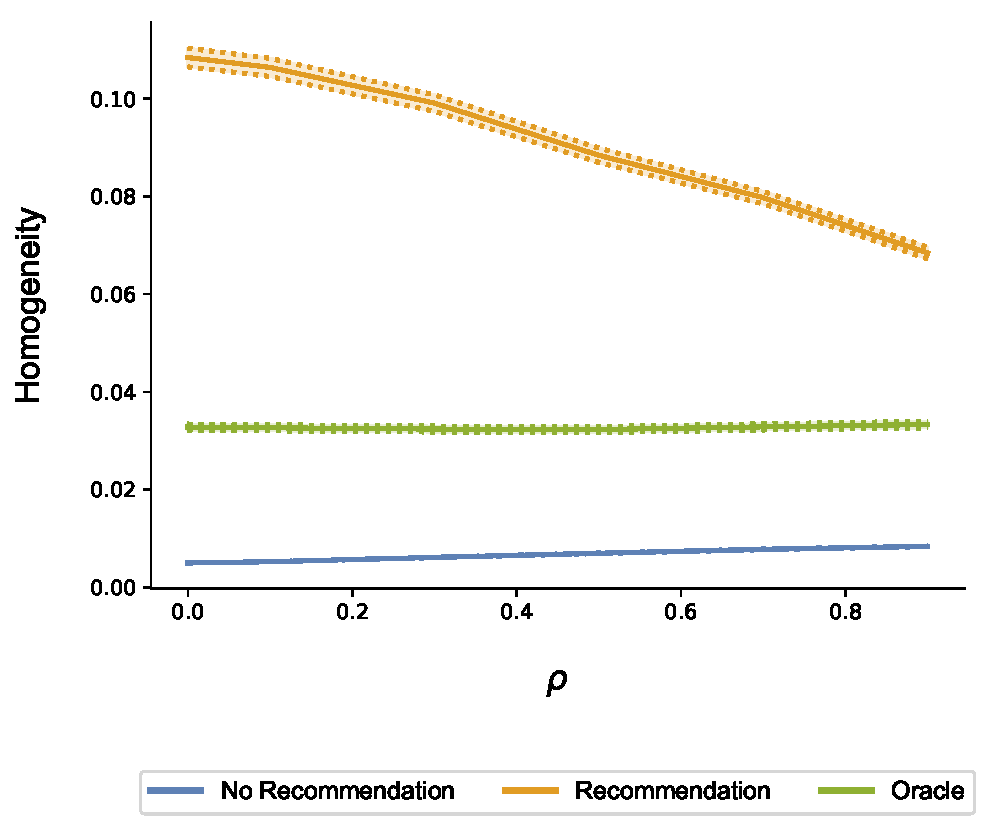
\includegraphics[scale=0.5]{rho_homogeneity_N_200_T_20}
\end{center}
\end{frame}
%
\begin{frame}{Towards Recommendation Design: \\Why are Accurate Recommendations not good?}
\begin{center}
    \begin{quote}
        Imagine you are using a travel recommender system.  
Suppose all of the recommendations it gives to you are 
for places you have already traveled to?  Even if the 
system was very good at ranking all of the places you 
have visited in order of preference, this still would be a 
poor recommender system.  Would you use such a 
system? 
    \end{quote}
    \vspace{0.5cm}
    - McNee, Riedhl, Konstan (2006)
    \end{center}
\end{frame}
%
\begin{frame}{Towards Recommendation System Design: \\Why are Accurate Recommendations not good?}
    \begin{itemize}
        \item Suppose the user liked \textit{John Wick}, should you recommend \textit{John Wick: Chapter Two}?
        \pause
        \item Recommender systems traditionally ignore inference users themselves make
        \begin{itemize}
            \item Good news - not useful information for user
            \item Bad news - useful information to users
        \end{itemize}
        \vspace{0.5cm}
        \textbf{Our approach}: Understanding user beliefs + how these evolve is a first-order component of designing useful recommendations
\end{itemize}
\end{frame}
%
\begin{frame}{Towards Recommendation System Design: \\ Serendipitous Recommendations}
One popular alternative design approach: \textbf{serendipity} 
\begin{quote}
\textit{A serendipitous recommendation helps the
user to find a surprisingly interesting item that
she might not have otherwise discovered (or it
would have been really hard to discover). [...]
Serendipity cannot happen if the user already
knows what is recommended to her, because a
serendipitous happening is by definition something new. Thus the lower is the probability that user knows an item, the higher is the probability that a specific item could result
in a serendipitous recommendation}.
\end{quote}
-Iaquinta, et. al (2010)
\pause
\begin{quote}
    Serendipitious recommendations should be simultaneously unexpected and useful
\end{quote}
-Maksai, et. al (2015)
\end{frame}
%
\begin{frame}{Towards Recommendation System Design: \\ Serendipitous Recommendations}
Two components of serendipitous recommendation:
\begin{enumerate}
    \item \textbf{Unexpected}: Depends on user beliefs - items that have low \textit{ex-ante} utility, given beliefs
    \item \textbf{Useful}: Induces users to take an action \textit{they wouldn't have taken without recommendation}
\end{enumerate}
\pause
\vspace{0.5cm}
    \textbf{Traditional approaches}: Predict \textit{ex-post} utilities and then try to ``diversify" the recommended itemset \\
    \vspace{0.5cm}
    \pause
    \textbf{Our approach}: Prediction problem should be estimating the marginal expected utility gain of providing information about particular items
\end{frame}
%
\begin{frame}{Conclusion}
\begin{itemize}
    \item Considered a model of long-lived users in the face of recommender systems
    \item Main takeaways:
    \begin{itemize}
        \item Model implies a clear path-dependence in choice
        \begin{itemize}
            \item Important for understanding the effects of platform steering and recommendation bias
        \end{itemize}
        \item Understanding user beliefs and how users learn over time crucial for both understanding the consequences of recommender systems and their design
    \end{itemize}
    \item Future directions:
    \begin{itemize}
        \item Designing recommender systems for long-lived consumers instead of a sequence of static problems
    \end{itemize}
\end{itemize}
\end{frame}
\end{document}
